\documentclass[12pt, letterpaper, titlepage]{article}

\usepackage{amsmath}
\usepackage{booktabs}
\usepackage{amsthm}
\usepackage{graphicx}
\usepackage[margin=1in]{geometry}
\usepackage{hyperref}
\hypersetup{colorlinks = true, linkcolor = blue, citecolor=blue, urlcolor = blue}
\usepackage{natbib}
\usepackage{enumitem}
\usepackage{setspace}

\usepackage[pagewise]{lineno}
%\linenumbers*[1]
% %% patches to make lineno work better with amsmath
\newcommand*\patchAmsMathEnvironmentForLineno[1]{%
 \expandafter\let\csname old#1\expandafter\endcsname\csname #1\endcsname
 \expandafter\let\csname oldend#1\expandafter\endcsname\csname end#1\endcsname
 \renewenvironment{#1}%
 {\linenomath\csname old#1\endcsname}%
 {\csname oldend#1\endcsname\endlinenomath}}%
\newcommand*\patchBothAmsMathEnvironmentsForLineno[1]{%
 \patchAmsMathEnvironmentForLineno{#1}%
 \patchAmsMathEnvironmentForLineno{#1*}}%

\AtBeginDocument{%
 \patchBothAmsMathEnvironmentsForLineno{equation}%
 \patchBothAmsMathEnvironmentsForLineno{align}%
 \patchBothAmsMathEnvironmentsForLineno{flalign}%
 \patchBothAmsMathEnvironmentsForLineno{alignat}%
 \patchBothAmsMathEnvironmentsForLineno{gather}%
 \patchBothAmsMathEnvironmentsForLineno{multline}%
}

% control floats
\renewcommand\floatpagefraction{.9}
\renewcommand\topfraction{.9}
\renewcommand\bottomfraction{.9}
\renewcommand\textfraction{.1}
\setcounter{totalnumber}{50}
\setcounter{topnumber}{50}
\setcounter{bottomnumber}{50}

\newcommand{\jy}[1]{\textcolor{blue}{JY: #1}}
\newcommand{\eds}[1]{\textcolor{red}{EDS: (#1)}}


\title{Sample Length at Which Block Bootstrapping is Effective for Estimation of Parameter of Time Series}

\author{Mathew Chandy\\
%   \href{mailto:mathew.chandy@uconn.edu}
% {\nolinkurl{mathew.chandy@uconn.edu}}\\
  Jun Yan\\[1ex]
  Department of Statistics, University of Connecticut\\
}
\date{}

\begin{document} 
\maketitle

\doublespace

\begin{abstract}
Block bootstrapping is a method that can be used for estimating a parameter of a time
series. It involves splitting a series into blocks (in order to account for the temporal dependence
factor) and re-sampling the blocks to create many new bootstrapped pseudo-samples of the time series.
This method becomes more effective as the length of the time series increases. 
The question that this study seeks to answer is what sample length is necessary for the block
bootstrap method to be effective in estimating a parameter of a time
series.

\bigskip
\noindent\sc{Keywords}:
block bootstrap;
\end{abstract}

\section{Introduction}
\label{sec:intro}

Block bootstrapping is a widely used method in Statistics. The concept for block 
bootstrapping was developed independently by \citet{hall1985resampling}, \citet{carlstein1986use}, and 
\citet{kunsch1989jackknife}. \citet{radovanov2014comparison} It has been applied to a variety of 
different domains such 
as econometrics \citep{mackinnon2006bootstrap} and meteorology \citep{varga2017generalised}. It can be used for 
situations in which there is temporal dependence within a population, and the goal is the estimation or testing a hypothesis about a parameter. Assuming that the sample is infinitely 
large, the method will work perfectly. However, for a finite sample size, the method will 
not work as well as expected. \citet{hesterberg2015teachers} notes that while percentile-based confidence intervals from nonparametric bootstrapping are more accurate than t-intervals for larger sample sizes, they are less accurate for smaller sample sizes. In the context of planning an applied 
statistical procedure, for which a large sample size is not always practical, it may be helpful to know how large the sample must be for the method to work at an acceptable level. 
The goal of this study is to find a threshold or range of sample sizes at which block bootstrap 
is an effective method for estimating a parameter. The method is effective if approximately 1 - $\alpha$/2 \% (for some predetermined significance level $\alpha$) of confidence intervals created from samples of the same size recover the parameter.

\citet{nevitt2001performance} find that a sample size of 200-1000 is usually sufficient for estimation using the bootstrap method (simple resampling with no blocks involved). However, in this study, the focus is block bootstrapping a temporally dependent sample.This is a different situation altogether, first, because the sample has a dependence factor that must be accounted for, and second because block bootstrapping involves splitting the sample into blocks.

\citet{goncalves2005bootstrap} found that standard error estimates from block bootstrapping small 
samples 
may be significantly more accurate than inference from closed-form asymptotic estimates. That study focused on the estimation of a coefficient parameter within the context of linear regression. Still, the block bootstrap percentile confidence intervals under-covered the parameter even for n = 1024. This study aims to find how small the sample size can be for a time series (which has a time dependence factor comparable to a coefficient of a linear regression) in order for the coverage rate to be close to the confidence level.

For this study, the block bootstrap method was applied to time series simulations in R. 

%At the base level, we are block-bootstrapping an auto-regressive process with true mean 0, and some AR(1) coefficient.

Bootstrapping is the procedure of creating new pseudo-samples of the same size by resampling observations with replacement from
the original sample. Basic bootstrapping works well for samples
that are do not have a dependence factor. However, for a time series such as an auto-regressive or moving-average process,
a different procedure is required to account for the time dependence. In such a situation, instead of resampling observations, blocks of the original sample can be resampled (these blocks must be of a certain length by which the sample length is divisible) to create a pseudo-sample. Point estimates of a parameter calculated from many block bootstrapped pseudo-samples are then used to create a distribution to create an interval estimation of the parameter.

%In this experiment, the mean, auto-correlation function (with a maximum lag of 1), and variance of a 1000 block-bootstrapped time series samples are computed, and 95\% confidence intervals of these parameters is created. 

The various ways which these intervals can be constructed are described in \citet{diciccio1996bootstrap} and \citet{rice2006mathematical}. They will be discussed later in a review of the block bootstrap method. For the purposes of this study (in which the true parameters are known), in order to establish whether or not the method is effective, the block bootstrapping of a simulated sample can be replicated many times, 
and the proportion of confidence intervals that recover the true known parameter 
(coverage rate) is recorded. The goal of this is simply to observe how successful the block bootstrapping procedure
is at estimating a parameter. The key variable being observed was, the sample length (n). It is known that as n
increases, block bootstrapping should become a more accurate and precise method for estimation
(the coverage rates will approach the theoretical confidence level and the interval widths will decrease). The question is what is the minimum sample length necessary to reach a coverage rate of 1 - $\alpha$/2 \%.

In this experiment, there are certain variables that are expected to affect the performance of block bootstrap. As the the time dependence (AR or MA coefficient) of the time series 
increases, we expect the coverage rates of the confidence intervals to decrease.
The coverage rates are also affected by the size of the blocks - more specifically,
how the size of the blocks (l) relates to the size of the time series (n) - 
and whether or not they overlap. It is known that as the size of the time series 
increases, the optimal block length should increase, and the ratio of the block length to 
the time series length should decrease. l = n$^{1/3}$ is typically considered the optimal 
block length according to asymptotic theory. \citep{buhlmann1999block} Therefore, simulations in this study were conducted using this optimal function of l = n$^{1/3}$. 

%In order to solve the question of what sample length is necessary for effective block bootstrapping while still accounting for all these factors, the simulations were repeated for different variations of the MA coefficient, target parameter, and non-moving vs moving method. 

For each of these variations, results for block bootstrap estimation of mean, MA coefficient, and standard deviation were recorded for a wide range of sample length.

\section{Review of Block Bootstrap}
\label{sec:blkbootreview}

Block bootstrapping is a method that can be applied to a non-stationary process to estimate a parameter. Suppose that a sample of length n of a time series is given. In regular bootstrap procedure, the new pseudo-sample of the same size as the original sample would be created by simply resampling observations from the with replacement. In the case of a time series, in order to account for the temporal dependence, the time series can be split into blocks, typically of the same size. The block should be of size l large enough to include time dependence, yet small enough to include some variance. l should also divide n. As n increases, an ideal l should also increase, but the ratio of l to n should decrease. To achieve this, l is often assigned a value as a function of n. A common function that is considered the best by much previous literature is l = n$^{1/3}$. To make things sample for this study, only perfect cubes were used for the sample length. A bootstrapped sample is created by taking a sample of n / l blocks with replacement to create a new pseudo-sample of size n. The designer of the study can choose whether the blocks overlap or not. If the blocks can never overlap, it is called a non-moving block bootstrap. In this case, the original sample is split evenly into n / l blocks, and the same number of blocks are sampled with replacement to create a bootstrapped pseudo-sample. If the blocks do overlap, it is called a moving block bootstrap. n / l samples are taken randomly from the original sample, but they do not have to be from a set of evenly spaced blocks. An estimate of the parameter (or parameters) is computed from the bootstrapped sample. This procedure can be repeated many times to create a sampling distribution of the estimator. In this study, 1000 bootstrapped pseudo-samples were created for each simulation. Using this distribution of point estimates, a 1 - $\alpha$/2 \% confidence interval for the parameter can be created. The most simplistic method for constructing this interval is the percentile confidence interval. For a parameter $\theta$, the percentile confidence interval takes the form: \[ [ ]\]. Another method for constructing this interval is the empirical confidence interval, which takes the form: \[ [ ]\]. The last method used in this study is the bias-corrected and accelerated 
(BCA) confidence interval, which takes the form: \[ [ ]\].

\section{Simulation Study Design}
\label{sec:simdesign}

The central objective of the study was to assess what sample size is necessary for the the block bootstrap method to estimate a parameter of an autoregressive process. The method will work better as the sample size goes to infinity, but the goal is to see what is the smallest sample size that is acceptable. The sample size is acceptable if many 1 - $\alpha$/2 confidence intervals for that sample size recover the parameter at a rate of 1 - $\alpha$/2. In the previous section, the procedure for creating a confidence interval of a parameter using the block bootstrap method is described. This process is applied to a simulation of an autoregressive integrated moving average (ARIMA) process to create a confidence interval of a certain parameter (could be the mean or the AR(1) coefficient). R has a built in ARIMA simulation which allows you to set the mean, AR(1) coefficient, and the standard deviation of the error term. Using the equation below, the standard deviation of the error term can be set so that the standard deviation of Y is constant (0.1, Variance = 0.01). 

\[ \sigma_{x}^{2}=\sigma_{\eta}^{2}/\left( 1-\phi^2 \right)\]
\[\sigma_{\eta}=\sqrt{\sigma_{x}^{2}*\left( 1-\phi^2 \right)}\]

For all simulation studies, the mean can be kept at 0, but the AR(1) Coefficient is the main factor that makes block bootstrap less effective, so its impact on the method's performance should be analyzed. For a certain variation of the ARIMA process, block bootstrap 95\% confidence intervals for each of 3 parameters (mean, AR(1) Coefficient, and sigma-squared) for a sample of length 32 is replicated 4000 times (each replication of the method is applied to a newly generated ARIMA simulation). For each individual confidence interval, it can be recorded whether or not the interval includes the true parameter. The coverage rate, or the proportion of intervals that include the true parameter, can then be recorded. If the parameter and its variance are being properly estimated by the block bootstrap, the coverage rate should reflect this by being close to the confidence level of 95\%. If this is not the case, the method is not working as well as it should. The width of the confidence interval for each replication is dependent on the variance of the parameter of the time series. If the interval is on average not wide enough to capture the parameter at the expected rate of 95\%, it indicates that the variance of the parameter (which will be estimated from the standard error of the parameter estimates from the bootstrapped samples) will be underestimated. If the interval is too wide and captures the parameter at a rate above 95\%, it indicates that the variance of the parameter will be overestimated. Since the coverage rate is a proportion based on many replication of independent Bernoulli outcomes, a 95\% confidence interval of the coverage rate at that sample size can also be created. We can be 95\% confident that the true expected coverage rate is included in this interval, so if .95 is included in the interval, this indicates that the block bootstrap method is working well. Once the simulation is done for this sample size, the process can be run again with a sample twice as big. This can be continued until the method is determined to be working acceptably (.95 is included within the confidence interval of the coverage rate).

\section{Methods}
\label{sec:methods}

6 variations of simulation studies were analyzed based on factors that might affect the results of the block bootstrap method. Simulation studies were conducted for an autoregressive process with AR = 0, an autoregressive process with AR = 0.2, and an autoregressive process with AR = 0.4. For each of these AR(1) coefficient values, separate simulation studies were conducted for the mean and AR(1) coefficient. For each of these variations, the non-moving block bootstrap method as well as the moving block bootstrap method were applied to estimate the respective parameter. 

The goal was to determine what range of sample sizes was acceptable for each of these variations of simulation studies. For theta = 0, results for five sample sizes (32, 64, 128, 256, 512) were observed. For theta = 0.2, results for eight sample sizes (32,  64, 128, 256, 512, 1024, 2048, 4096) were observed. For theta = 0.4, results for nine sample sizes (32, 64, 128, 256, 512, 1024, 2048, 4096, 8192) were observed.



 

\section{Results}
\label{sec:results}

As the AR(1) coefficient increases, it was found unsurprisingly that a large sample size was needed for the block bootstrap method to work. When the target for estimation was the mean or the variance of the process, moving block bootstrap generally had a similar performance to non-moving block bootstrap. However when the target for estimation was the AR(1) coefficient of the process, moving block bootstrap noticeably recovered the parameter at a greater rate than non-moving block bootstrap. When the target was the mean or the variance and theta was more than 0, the coverage rate was generally much higher than that for when the target was the AR(1) coefficient. However when theta was 0, the AR(1) coefficient was recovered at a greater rate than the mean or variance . 



\begin{figure}[tbp]
\caption{The figure below shows results for block bootstrap estimation when theta is 0. When the target was the mean and the moving method was used, the coverage rate confidence interval included .95 when the sample length was 512, indicating that even for a sample with no temporal dependence, a very large sample length of around 500 is necessary to get an accurate estimation of the mean. Similarly, when the target was the mean and the non-moving method was used, the coverage rate confidence interval included .95 when the sample length was 512, showing that a sample size of around 500 is necessary for good block bootstrap estimation. When the target was the AR(1) coefficient and the moving method was used, the parameter was over-covered - all of the coverage rate confidence interval lower bounds were greater than .95 - for all sample sizes that were observed (32, 64, 128, 256, and 512). This indicates that the variance of the parameter is being overestimated. When the target was the AR(1) coefficient and the non-moving method was used, the parameter was under-covered when the sample length was 32 and slightly over-covered when the sample length was 256. For sample lengths 64, 128, and 512, the non-moving method recovered the parameter well.}
  \centering
  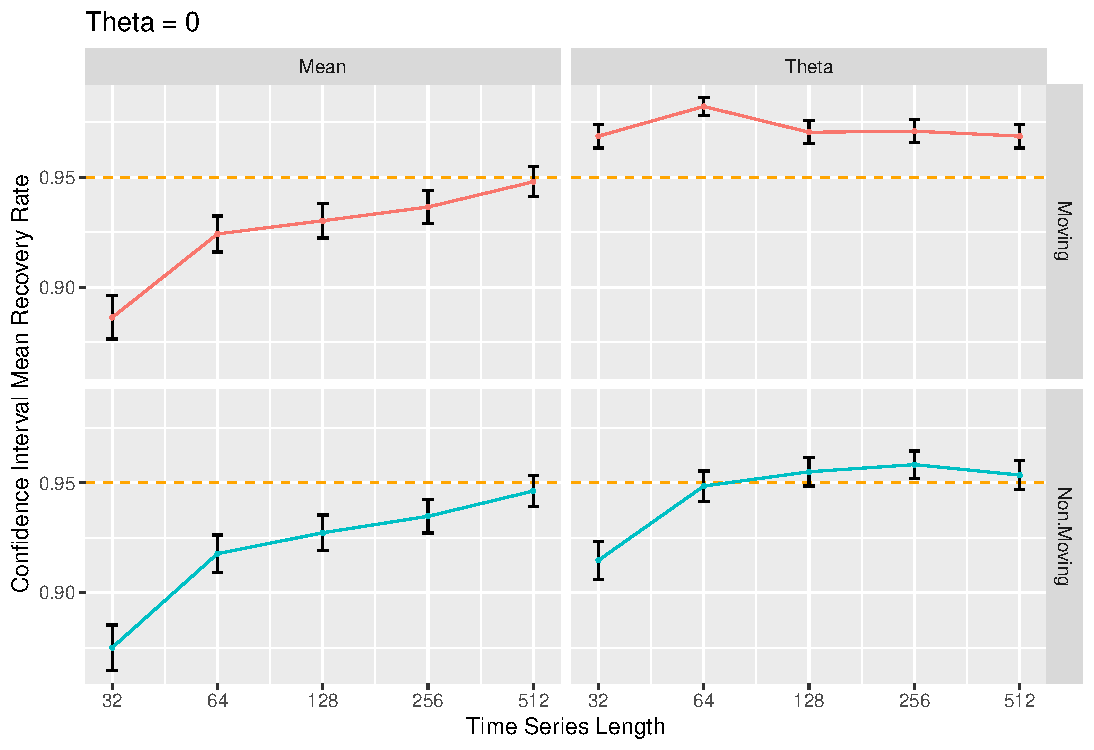
\includegraphics[width=\textwidth]{theta_0}
  \caption{}
  \label{fig:theta_0}
\end{figure}

\begin{figure}[tbp]
\caption{The figure below shows results for block bootstrap estimation when theta is 0.2. When the target was the mean and the moving method was used, the coverage rate confidence interval included .95 when the sample length was 2048 and 4096, indicating that even for a sample with relatively low temporal dependence, a very large sample of around 2000 is necessary to get an accurate estimation of the mean. Similarly, when the target was the mean and the non-moving method was used, the coverage rate confidence interval included .95 when the sample length was 2048 and 4096, showing that a sample size of around 2000 is necessary for good block bootstrap estimation. When the target was the AR(1) coefficient, for both methods, the parameter was under-covered for sample lengths as large as 4096, although the moving method appeared to perform better for all sample sizes. }
  \centering
  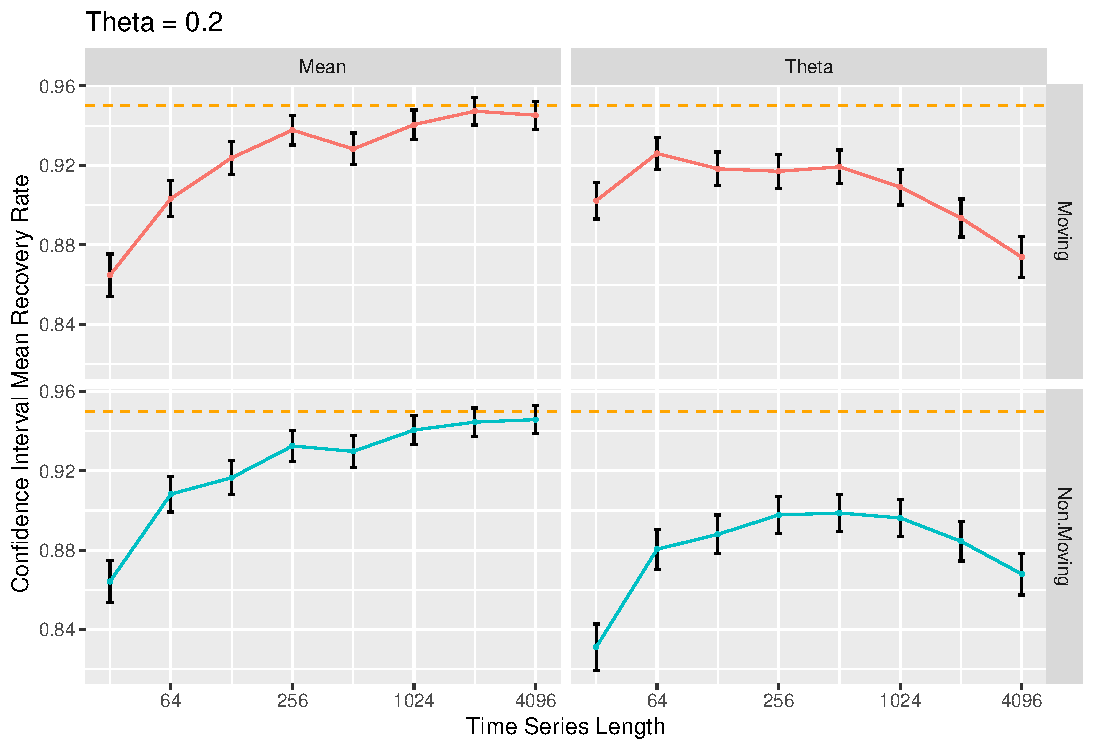
\includegraphics[width=\textwidth]{theta_0.2}
  \caption{}
  \label{fig:theta_0.2}
\end{figure}

\begin{figure}[tbp]
\caption{The figure below shows results for block bootstrap estimation when theta is 0.4. When the target was the mean, for both methods, the coverage rate was under-covered for sample sizes as large as 8192. When the target was the AR(1) coefficient, for both methods, the parameter was under-covered for sample lengths as large as 4096, although the moving method appeared to perform better for smaller sample sizes. }
  \centering
  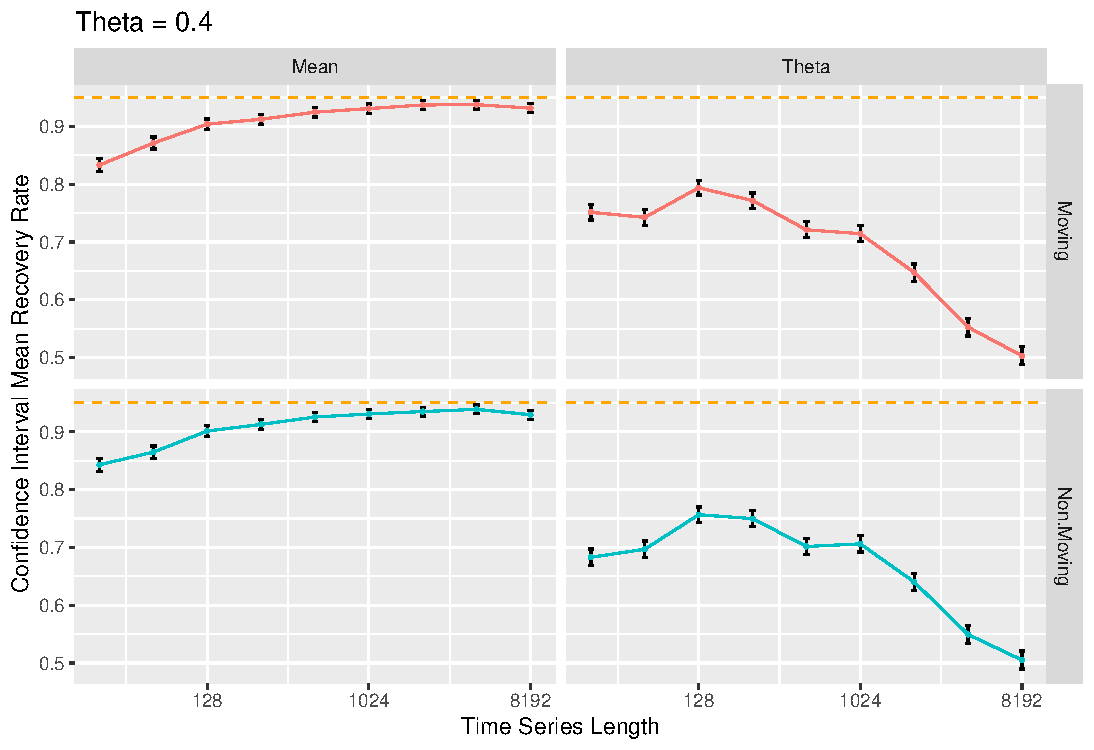
\includegraphics[width=\textwidth]{theta_0.4}
  \caption{}
  \label{fig:theta_0.4}
\end{figure}

\section{Discussion}
\label{sec:discuss}

This study finds that as the AR coefficient increases, the sample size necessary for effective block bootstrap estimation must be larger. When implementing the block bootstrap method to estimate the mean or variance of an autoregressive process, the non-moving method and moving method perform about the same. However, when estimating the AR(1) coefficient, the non-moving method performs noticeably worse than the moving method, which still covers the coefficient poorly when theta is greater than 0. Whereas the performance improves as sample length increases when the target is the mean or variance, the performance decays as sample length increases when the target is the AR(1) coefficient.



\bibliographystyle{chicago}
\bibliography{citations}[tp]


\end{document}